\chapter{仿真实验与结果分析}
针对上述方法,对无人机轨迹规划方法进行仿真实验。首先在 MATLAB 上证明了优化策略的可行性,然后基于标准的无人机仿真框架搭建了仿真环境,设计了仿真流程,完成了 ROS、PX4、Gazebo 的联合仿真内容。
\section{MATLAB 平台}
\subsection{规划算法验证}
在MATLAB平台上验证路径搜索算法,在之前获得的速度场的基础上进行波形传播和速度搜索,图 \ref{fig_pathtimereal2} 为搜索出来的路径和到达时间图。

\begin{figure}[H]
    \centering
    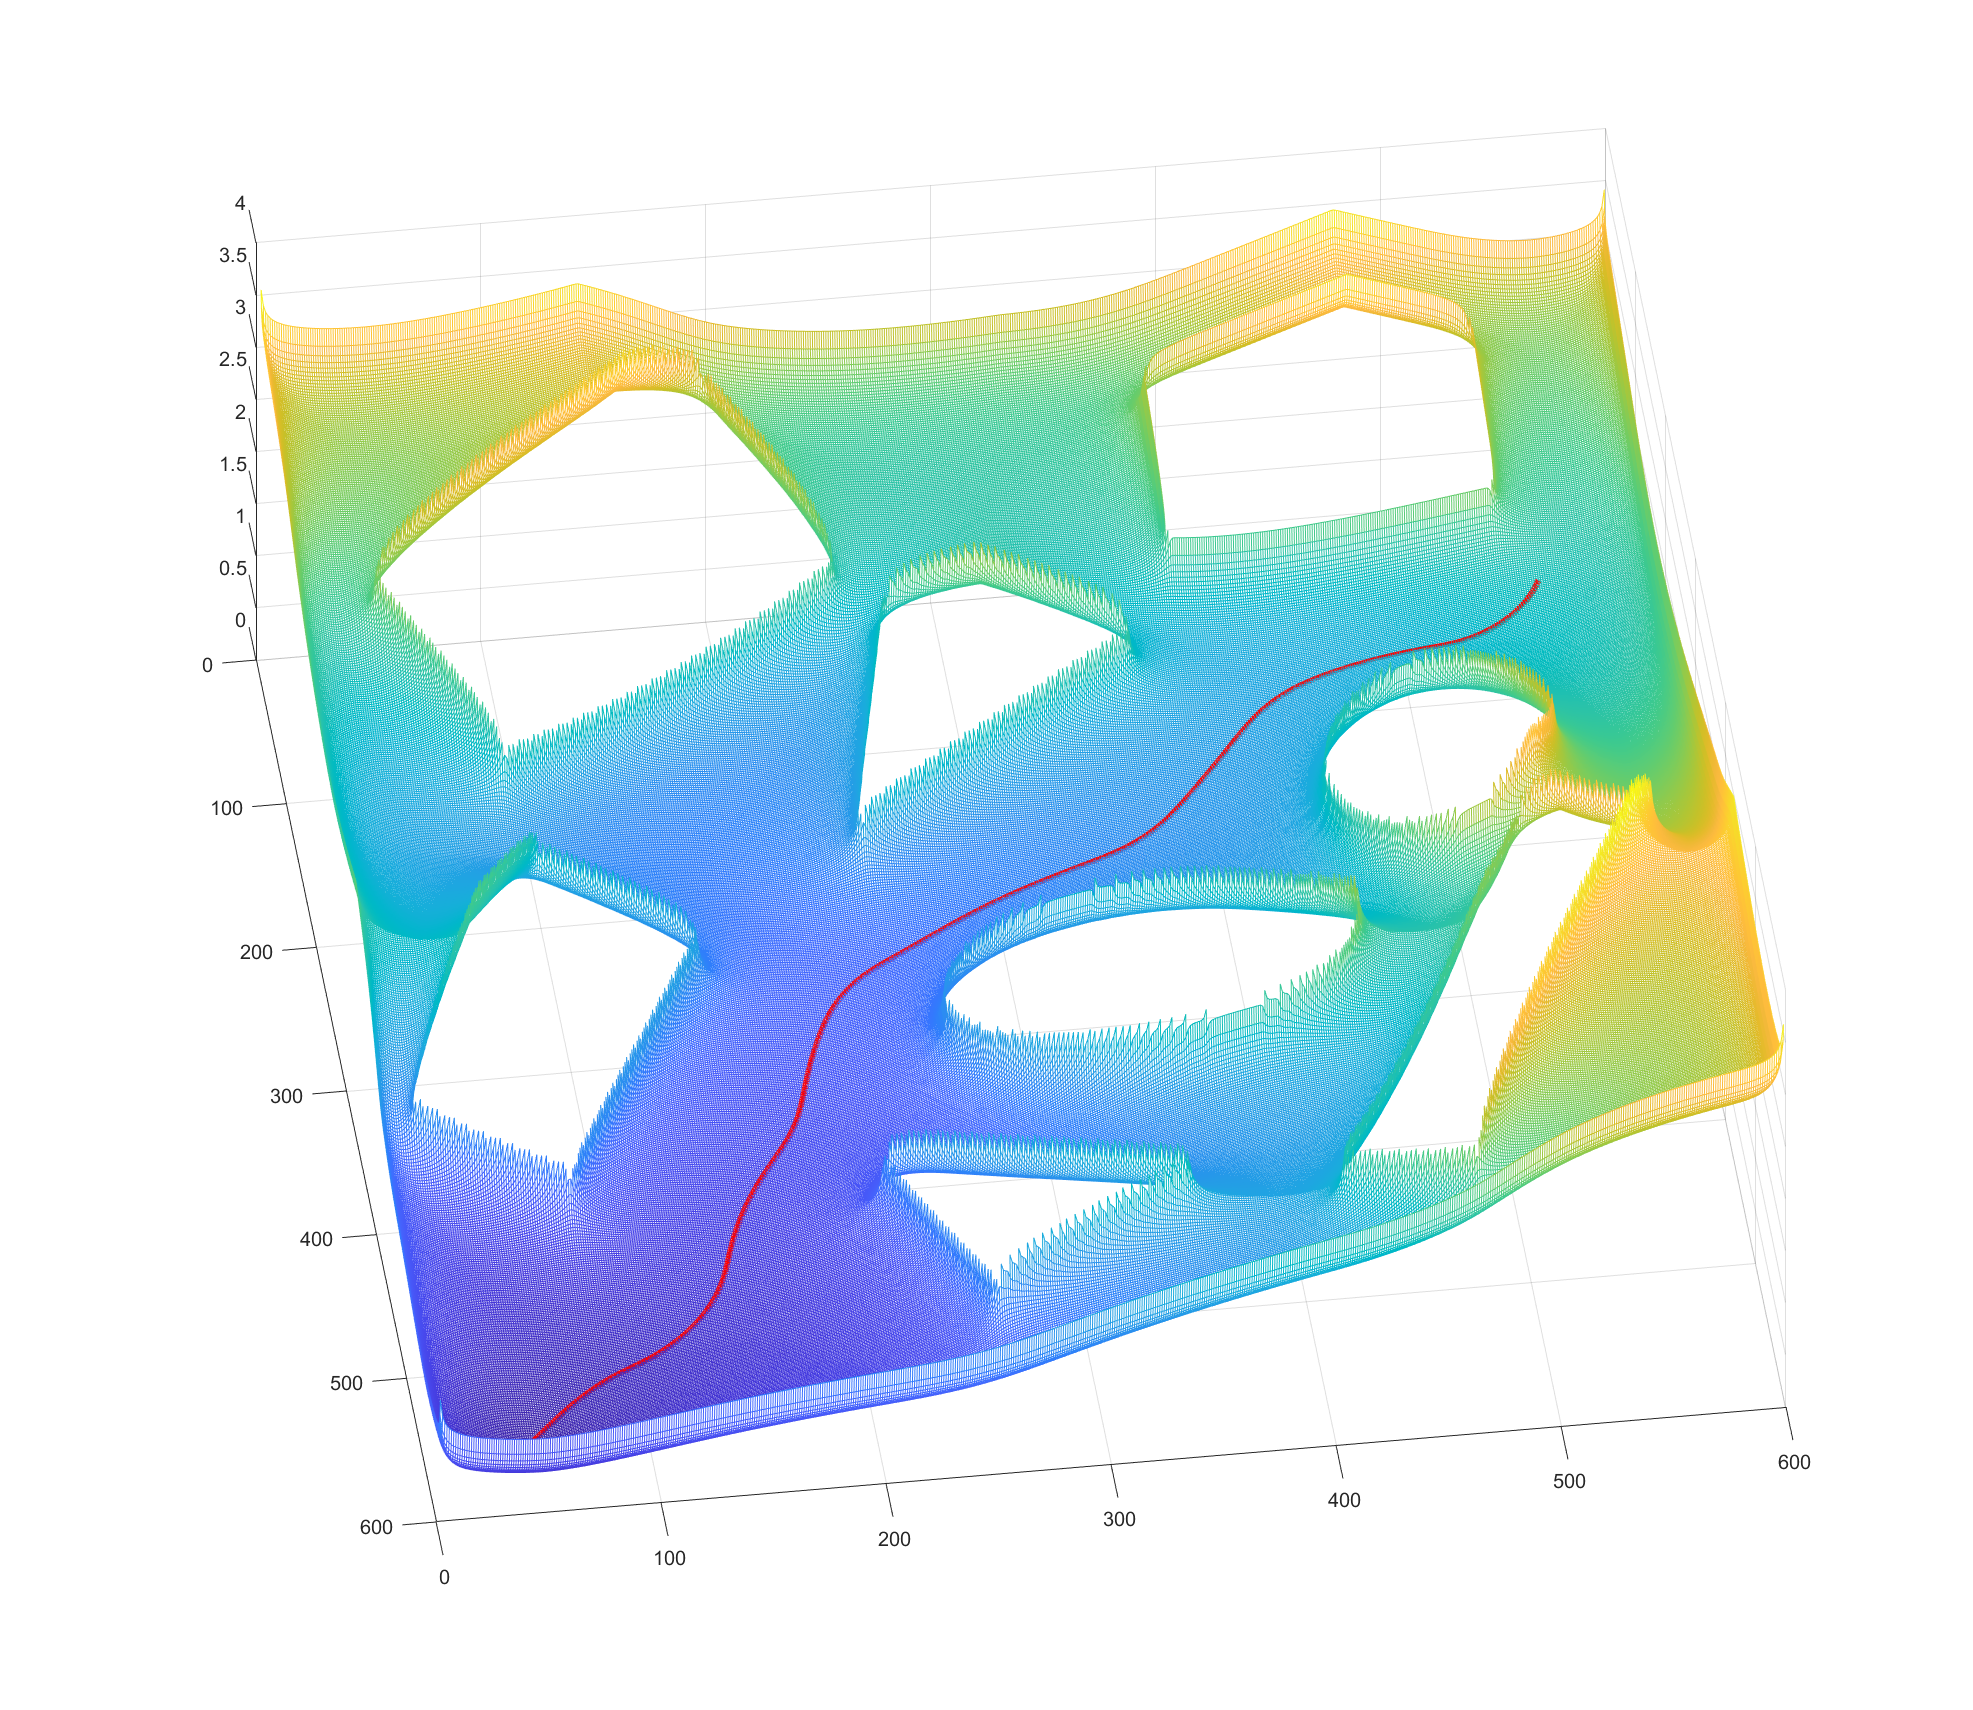
\includegraphics[width=12cm]{figures/fig_pathtimereal.png}
    \caption{
        路径和到达时间图
    }
    \label{fig_pathtimereal2}
\end{figure}

\begin{table}[H]
    \centering
    \caption{参数设置}
    \label{form_2}
    \begin{tabular}{cccccc}
    \hline
    \multirow{2}{*}{多项式阶数} & \multicolumn{2}{c}{最大速度限制} & \multicolumn{2}{c}{最大加速度限制} & \multirow{2}{*}{分段轨迹时间}       \\ \cline{2-5}
                           & x            & y           & x            & y            &                                                                                               \\ \hline
    5                      & 5m/s         & 5m/s        & 2 $m^2$/s       & 2 $m^2$/s       & \begin{tabular}[c]{@{}c@{}}{[}16.50;16.50;16.50;\\   16.50;16.50;16.50{]}(s)\end{tabular} \\ \hline
    \end{tabular}
\end{table}

表格可用https://www.tablesgenerator.com/ 在线工具转换
\endinput